\documentclass[tikz, border=20pt]{standalone}
\usepackage[utf8]{inputenc}
\usepackage{helvet}
\renewcommand{\familydefault}{\sfdefault}
\usetikzlibrary{positioning, shapes.geometric, arrows.meta, calc, fit, backgrounds}

\begin{document}
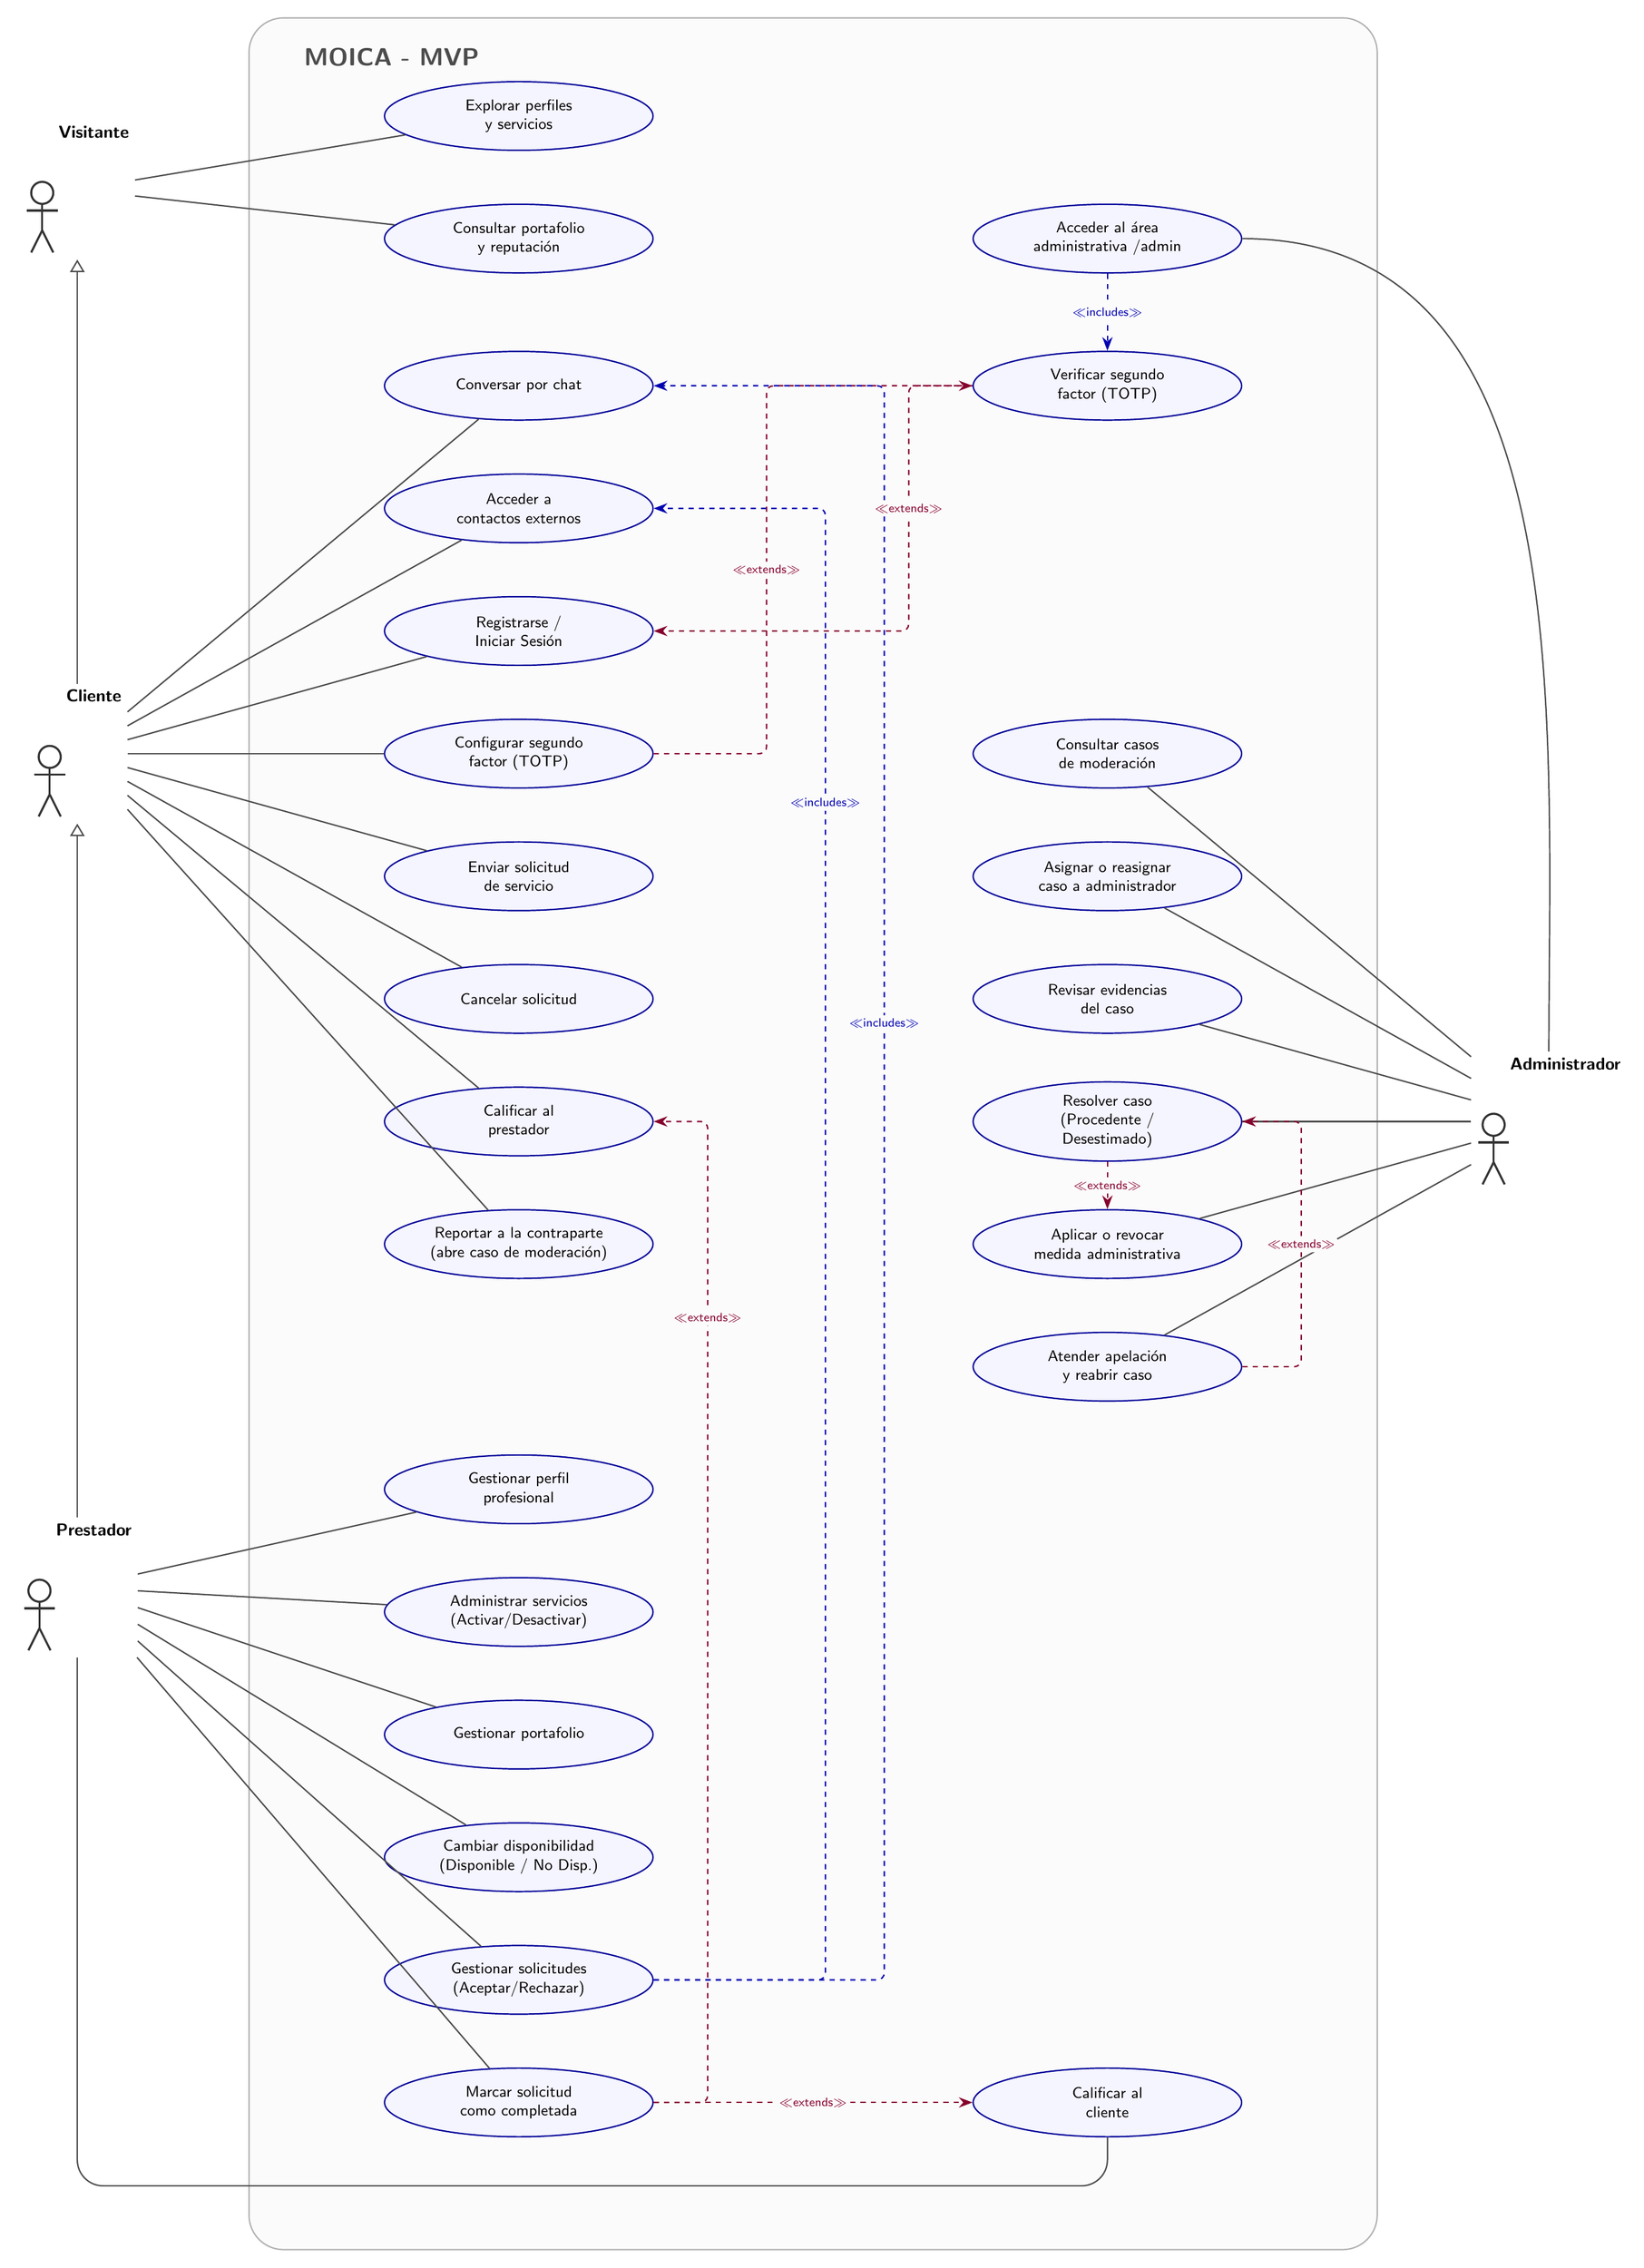
\begin{tikzpicture}[
    actor/.style={
        align=center, font=\bfseries\sffamily,
        execute at begin node={
            \tikz[scale=0.45, line width=1.2pt, baseline=1.8cm, color=black!80]{
                \draw (0,1.5) circle (0.5);
                \draw (0,1) -- (0,-0.2);
                \draw (-0.7,0.7) -- (0.7,0.7);
                \draw (0,-0.2) -- (-0.5,-1.2);
                \draw (0,-0.2) -- (0.5,-1.2);
            }\\[0.5ex]
        }
    },
    usecase/.style={
        ellipse, draw=blue!60!black, thick, fill=blue!4,
        minimum width=4.8cm, minimum height=1.4cm,
        align=center, font=\small\sffamily, text width=3.8cm,
        inner sep=1pt
    },
    system/.style={
        rectangle, draw=black!30, thick, fill=gray!3,
        rounded corners=20pt, inner sep=0pt
    },
    assoc/.style={thick, draw=black!70},
    inherit/.style={thick, draw=black!70, -{Triangle[open, scale=1.5]}},
    include/.style={dashed, thick, draw=blue!70!black, -{Stealth[scale=1.2]}},
    extend/.style={dashed, thick, draw=purple!70!black, -{Stealth[scale=1.2]}}
]

% ====================
% LÍMITE DEL SISTEMA
% ====================
\draw[system] (1.5, -19.5) rectangle (24.5, 26);
\node[below right, font=\Large\bfseries\sffamily, text=black!70] at (2.5, 25.5) {MOICA - MVP};

% ====================
% ACTORES
% ====================
\node[actor] (V) at (-2, 22.5) {Visitante};
\node[actor] (C) at (-2, 11) {Cliente};
\node[actor] (P) at (-2, -6) {Prestador};
\node[actor] (A) at (28, 3.5) {Administrador};

% Herencia de actores
\draw[inherit] (C) -- (V);
\draw[inherit] (P) -- (C);

% ====================
% CASOS DE USO
% ====================

% --- Columna Central (Visitante, Cliente, Prestador) ---
\node[usecase] (UC_Exp) at (7, 24) {Explorar perfiles\\y servicios};
\node[usecase] (UC_Con) at (7, 21.5) {Consultar portafolio\\y reputación};

\node[usecase] (UC_Cha) at (7, 18.5) {Conversar por chat};
\node[usecase] (UC_ConEx) at (7, 16) {Acceder a\\contactos externos};
\node[usecase] (UC_Log) at (7, 13.5) {Registrarse /\\Iniciar Sesión};
\node[usecase] (UC_Conf2FA) at (7, 11) {Configurar segundo\\factor (TOTP)};
\node[usecase] (UC_Env) at (7, 8.5) {Enviar solicitud\\de servicio};
\node[usecase] (UC_Can) at (7, 6) {Cancelar solicitud};
\node[usecase] (UC_CalP) at (7, 3.5) {Calificar al\\prestador};
\node[usecase] (UC_Rep) at (7, 1) {Reportar a la contraparte\\(abre caso de moderación)};

\node[usecase] (UC_GP) at (7, -4) {Gestionar perfil\\profesional};
\node[usecase] (UC_GS) at (7, -6.5) {Administrar servicios\\(Activar/Desactivar)};
\node[usecase] (UC_GPo) at (7, -9) {Gestionar portafolio};
\node[usecase] (UC_Disp) at (7, -11.5) {Cambiar disponibilidad\\(Disponible / No Disp.)};
\node[usecase] (UC_AR) at (7, -14) {Gestionar solicitudes\\(Aceptar/Rechazar)};
\node[usecase] (UC_Comp) at (7, -16.5) {Marcar solicitud\\como completada};

% --- Columna Derecha (Calificar al cliente y Administrador) ---
\node[usecase] (UC_CalC) at (19, -16.5) {Calificar al\\cliente};

\node[usecase] (UC_Adm) at (19, 21.5) {Acceder al área\\administrativa /admin};
\node[usecase] (UC_2FA) at (19, 18.5) {Verificar segundo\\factor (TOTP)};

\node[usecase] (UC_CRep) at (19, 11) {Consultar casos\\de moderación};
\node[usecase] (UC_Asig) at (19, 8.5) {Asignar o reasignar\\caso a administrador};
\node[usecase] (UC_RevE) at (19, 6) {Revisar evidencias\\del caso};
\node[usecase] (UC_ResR) at (19, 3.5) {Resolver caso\\(Procedente / Desestimado)};
\node[usecase] (UC_EmiM) at (19, 1) {Aplicar o revocar\\medida administrativa};
\node[usecase] (UC_Apel) at (19, -1.5) {Atender apelación\\y reabrir caso};


% ====================
% ASOCIACIONES
% ====================

% Visitante
\draw[assoc] (V) -- (UC_Exp);
\draw[assoc] (V) -- (UC_Con);

% Cliente
\draw[assoc] (C) -- (UC_Cha);
\draw[assoc] (C) -- (UC_ConEx);
\draw[assoc] (C) -- (UC_Log);
\draw[assoc] (C) -- (UC_Conf2FA);
\draw[assoc] (C) -- (UC_Env);
\draw[assoc] (C) -- (UC_Can);
\draw[assoc] (C) -- (UC_CalP);
\draw[assoc] (C) -- (UC_Rep);

% Prestador
\draw[assoc] (P) -- (UC_GP);
\draw[assoc] (P) -- (UC_GS);
\draw[assoc] (P) -- (UC_GPo);
\draw[assoc] (P) -- (UC_Disp);
\draw[assoc] (P) -- (UC_AR);
\draw[assoc] (P) -- (UC_Comp);
% Rutada ortogonalmente por debajo para no cruzar los casos de uso
\draw[assoc, rounded corners=15pt] (P) -- (-2, -18.2) -| (UC_CalC.south);

% Administrador
\draw[assoc] (A) to[out=90, in=0] (UC_Adm.east);
\draw[assoc] (A) -- (UC_CRep);
\draw[assoc] (A) -- (UC_Asig);
\draw[assoc] (A) -- (UC_RevE);
\draw[assoc] (A) -- (UC_ResR);
\draw[assoc] (A) -- (UC_EmiM);
\draw[assoc] (A) -- (UC_Apel);


% ====================
% INCLUDES / EXTENDS
% ====================

% UC_Adm includes UC_2FA (Línea recta vertical)
\draw[include] (UC_Adm.south) -- node[pos=0.5, fill=gray!3, font=\scriptsize\sffamily, text=blue!70!black, inner sep=2pt] {$\ll$\textsf{includes}$\gg$} (UC_2FA.north);

% UC_ResR extends UC_EmiM (Línea recta vertical)
\draw[extend] (UC_ResR.south) -- node[pos=0.5, fill=gray!3, font=\scriptsize\sffamily, text=purple!70!black, inner sep=2pt] {$\ll$\textsf{extends}$\gg$} (UC_EmiM.north);

% UC_Comp extends UC_CalC (Línea recta horizontal)
\draw[extend] (UC_Comp.east) -- node[pos=0.5, fill=gray!3, font=\scriptsize\sffamily, text=purple!70!black, inner sep=2pt] {$\ll$\textsf{extends}$\gg$} (UC_CalC.west);


% --- RUTAS ORTOGONALES EVITANDO SUPERPOSICIÓN (Bus Vertical) ---

% Carril 1: UC_Comp extends UC_CalP
\coordinate (V1) at ($(UC_Comp.east) + (1.1, 0)$);
\coordinate (V2) at (V1 |- UC_CalP.east);
\draw[extend, rounded corners] (UC_Comp.east) -- (V1) -- node[pos=0.8, fill=gray!3, font=\scriptsize\sffamily, text=purple!70!black, inner sep=2pt] {$\ll$\textsf{extends}$\gg$} (V2) -- (UC_CalP.east);

% Carril 2: UC_Conf2FA extends UC_2FA
\coordinate (V3) at ($(UC_Conf2FA.east) + (2.3, 0)$);
\coordinate (V4) at (V3 |- UC_2FA.west);
\draw[extend, rounded corners] (UC_Conf2FA.east) -- (V3) -- node[pos=0.5, fill=gray!3, font=\scriptsize\sffamily, text=purple!70!black, inner sep=2pt] {$\ll$\textsf{extends}$\gg$} (V4) -- (UC_2FA.west);

% Carril 3: UC_AR includes UC_ConEx
\coordinate (V5) at ($(UC_AR.east) + (3.5, 0)$);
\coordinate (V6) at (V5 |- UC_ConEx.east);
\draw[include, rounded corners] (UC_AR.east) -- (V5) -- node[pos=0.8, fill=gray!3, font=\scriptsize\sffamily, text=blue!70!black, inner sep=2pt] {$\ll$\textsf{includes}$\gg$} (V6) -- (UC_ConEx.east);

% Carril 4: UC_AR includes UC_Cha
\coordinate (V7) at ($(UC_AR.east) + (4.7, 0)$);
\coordinate (V8) at (V7 |- UC_Cha.east);
\draw[include, rounded corners] (UC_AR.east) -- (V7) -- node[pos=0.6, fill=gray!3, font=\scriptsize\sffamily, text=blue!70!black, inner sep=2pt] {$\ll$\textsf{includes}$\gg$} (V8) -- (UC_Cha.east);

% Carril 5: UC_2FA extends UC_Log
\coordinate (V9) at ($(UC_2FA.west) + (-1.3, 0)$);
\coordinate (V10) at (V9 |- UC_Log.east);
\draw[extend, rounded corners] (UC_2FA.west) -- (V9) -- node[pos=0.5, fill=gray!3, font=\scriptsize\sffamily, text=purple!70!black, inner sep=2pt] {$\ll$\textsf{extends}$\gg$} (V10) -- (UC_Log.east);


% --- RUTAS EXTERNAS ---

% UC_Apel extends UC_ResR (rodeando por la derecha para no cruzar UC_EmiM)
\coordinate (V11) at ($(UC_Apel.east) + (1.2, 0)$);
\coordinate (V12) at (V11 |- UC_ResR.east);
\draw[extend, rounded corners] (UC_Apel.east) -- (V11) -- node[pos=0.5, fill=gray!3, font=\scriptsize\sffamily, text=purple!70!black, inner sep=2pt] {$\ll$\textsf{extends}$\gg$} (V12) -- (UC_ResR.east);

\end{tikzpicture}
\end{document}